\chapter{Существующие подходы к созданию DSM-решений}
В этой главе рассматриваются существующие результаты, схожие с полученными в рамках 
данной диссертации, приводится позиционирование данной работы относительно этих результатов.

\section{Фокус и структура обзора}
Поскольку основным предметом исследований в данной работе является методология создания 
визуальных предметно-ориентированных языков, то обзор будет состоять из, во-первых, 
рассмотрения существующих теоретических работ, связанных с методологией, и во-вторых, 
обзора существующих инструментальных средств для создания визуальных языков.

Как ни странно, вопросам методологии создания визуальных языков уделялось внимание 
значительно меньшее, чем текстовых. В случае с текстовыми предметно-ориентированными
языками существуют подробные и обстоятельные работы, описывающие как жизненный цикл
языка, так и основные деятельности, которые должны быть выполнены на каждом этапе
жизненного цикла (такие, как \cite{mernik2005and} и обзор \cite{van2000domain}), в 
случае с визуальными языками, как правило, имеется лишь набор слабо структурированных
советов, рекомендаций и наблюдений, полученных из практики (наиболее подробное изложение 
можно найти в \cite{kelly2008domain}, также хорошим примером таких работ может послужить 
\cite{voelter2009best} или \cite{luoma2004defining}). Поэтому в обзор войдут и статьи, 
относящиеся к текстовым языкам --– вопросы реализации предметно-ориентированных средств 
разработки для текстовых языков для данной работы нерелевантны, но общая модель жизненного 
цикла языка, деятельности по анализу предметной области, некоторые аспекты проектирования 
языка, и подобные могут быть переиспользованы при разработке визуальных языков практически 
без изменений. Разумеется, нам будут интересны и статьи, содержащие опыт разработки 
визуальных языков, пусть и слабоструктурированный, поскольку они могут послужить базисом 
для создания методологии разработки. По этим же причинам в обзор будут включены статьи, 
в которых обсуждаются аспекты организации языковой инфраструктуры (например, \cite{atkinson2003model}) 
--– различные точки зрения на внутреннюю структуру и устройство визуальных языков 
могут приводить к необходимости выполнения разных действий при их создании.

Также значительное внимание в обзоре будет уделено существующим инструментальным средствам, 
аналогам системы QReal. Поскольку данная работа посвящена процессу создания визуальных 
языков, особенности инструментальных средств, к этому процессу непосредственно не 
относящиеся, рассматриваться не будут.
%TODO: ссылка на диссер Тимофея?
Большинство имеющихся описаний инструментальных средств не фокусируются на какой-либо методологии создания визуального языка (представляя 
cредства, но не указания по их использованию). В тех редких случаях, когда это не так, 
и инструментальное средство имеет за собой чёткую методологию его применения (как, 
например, в работе \cite{repenning1995agentsheets}), такое описание будет рассмотрено в 
первой части обзора, вместе с работами, излагающими общие методологические указания.

Существующих инструментальных средств создания предметно-ориентированных визуальных 
языков много, однако опыт в этой области программной инженерии практически не переиспользуется 
(что отмечают и авторы \cite{kelly2008domain}). Например, в обзоре будет упомянута 
система, публикация по которой датируется 1977 годом, имеющая все признаки типичной 
DSM-платформы (\cite{teichroew1977psl}), тогда как сам термин "`предметно-ориентированное 
моделирование"' (Domain-Specific Modeling) начал упоминаться в литературе начиная примерно с 
1995 года, 
%TODO: Звучит депрессивно, а мне бы следовало выражать энтузиазм по поводу DSL.
причём до сих пор данный подход во многих работах преподносится как новый, активно 
развивающийся и перспективный. Поэтому средства будут рассматриваться не в хронологическом 
порядке, а в порядке частоты их упоминаний в литературе, от наиболее часто упоминаемых к менее 
известным, насколько может судить автор данной работы.

В данном обзоре не будут рассмотрены работы, доказывающие экономическую целесообразность
применимости предметно-ориентированного подхода и визуального моделирования вообще,
ссылки на них читатель может найти во введении к диссертации. Кроме того, не будут
рассмотрены работы, в которых вводятся различные определения, относящиеся к визуальным
предметно-ориентированным языкам, классификации языков и т.д., имеющие лишь вспомогательное
значение для диссертации, ссылки на такие работы содержатся в главе \ref{chapter1}.

\section{Существующие методики и приёмы разработки предметно-ориентированных языков}
\subsection{Модели жизненного цикла языка}
\label{lifecycleModels}
Начать следует с общих вопросов жизненного цикла предметно-ориентированных языков.
В данном случае не имеет особого значения, визуальные это языки или текстовые, поскольку
различия между ними играют существенную роль лишь при реализации. Наиболее обстоятельное,
насколько нам известно, обсуждение данных вопросов приводится в статье \cite{mernik2005and}. 
Авторы выделяют следующие фазы существования предметно-ориентированного языка: принятие 
решения (о необходимости создания DSL), анализ (предметной области), проектирование 
(переиспользование языка общего назначения для создания DSL и спецификация DSL), реализация 
и развёртывание. Рекомендации по деятельности коллектива разработчиков на каждой фазе 
даны в виде паттернов с примерами применения в реальных проектах. 

В фазе принятия решения наиболее интересными для нас показателями применимости DSM-подхода могут служить: 
\begin{itemize}
	\item наличие сложного интерфейса прикладных программ (API), который можно было 
		бы представить сущностями созданного языка;
	\item наличие необходимости (или возможности) предметно-ориентированного анализа, 
		верификации, оптимизации, параллелизации и трансформации (авторами используется 
		акроним AVOPT, образованный первыми буквами английских эквивалентов перечисленных 
		терминов), которые требуют знания особенностей предметной области и поэтому неосуществимы 
		на языке общего назначения (авторы используют термин GPL, General Purpose Language);
	\item наличие семейства программных продуктов, имеющего довольно много общих частей 
		и некоторые различия, которые могут быть выражены посредством DSL;
	\item представление сложных структур данных и работа с ними.
\end{itemize}

На фазе анализа в основном применяются неформальные методы, хотя авторы упоминают 
несколько существующих формальных методологий (перечислены методологии
%TODO: ссылки
DARE, DSSA, FAST, FODA, ODE, ODM). Авторы отмечают отсутствие поддержки анализа предметной 
области в имеющихся инструментальных средствах, и из дальнейшего обзора станет ясно, 
что с визуальными предметно-ориентированными языками ситуация обстоит аналогичным 
образом. Существуют отдельные инструменты, поддерживающие формальный анализ предметной 
области, но ни один из них не интегрирован со средствами разработки языков, хотя анализ 
предметной области является входом для наиболее важной при создании предметно-ориентированного 
языка деятельности –-- выделения основных сущностей языка.

Паттерны фаз проектирования и реализации, описанные в статье, оказываются если не полностью 
неприменимы к визуальным языкам, то достаточно далеки от применяемых в случае визуальных 
языков подходов, чтобы было необходимо рассматривать другие источники. Действительно, 
авторы выделяют переиспользование языка общего назначения при создании DSL как один 
из возможных подходов к проектированию, и для визуальных языков это тоже может быть 
применимо, например, использование механизмов расширения языка UML, но это отдельная 
тема, которая заслуживает отдельного обсуждения. Подходы, типичные для этих фаз, будут 
обсуждаться далее при рассмотрении более подходящих для этого источников.

В статье совершенно не рассматриваются аспекты существования языка после его развёртывания, 
что довольно странно, поскольку редко бывает, чтобы язык был сразу же создан таким, 
каким его было бы удобно использовать. Эволюция предметно-ориентированного языка требует 
особого рассмотрения, поскольку должна осуществляться совместно с созданными на этом языке 
моделями (или программами), и её нельзя исключать из модели жизненного цикла. Интересные 
в контексте данной работы выводы, сделанные в статье –-- существующие инструментальные средства 
фокусируются в основном на вопросах реализации и либо не предоставляют вообще средств 
автоматизации других фаз жизненного цикла, либо эта поддержка весьма ограничена. 

Работа \cite{van2000domain} интересна сама по себе как подробная библиография, посвящённая 
текстовым предметно-ориентированным языкам, покрывающая вопросы терминологии, целесообразности 
использования DSL, методологии создания, реализации DSL, и содержащая ссылки на массу 
примеров. Для нас существенны вопросы методологии. Авторы делят фазы жизненного цикла языка 
на три группы --- анализ, реализация и использование. Этап анализа, как и в предыдущей работе, 
предполагает применение неформального подхода или одной из формальных методик (здесь их 
применение называется инженерией предметной области, или domain engineering), кроме 
того, в качестве источника информации для анализа указываются унаследованные системы 
(legacy systems), либо существующие библиотеки или каркасы приложений. Реализация 
рассмотрена исключительно для текстовых языков, информации по последнему этапу жизненного 
цикла --- использованию языка --- не представлено.

Работы \cite{koznov2011process} и \cite{koznov2008development} рассматривают процесс 
разработки языка с менее технической точки зрения. Предлагается в качестве модели 
для разработки DSM-решения в небольших и средних компаниях использовать методологию 
Microsoft Solution Framework (MSF), несколько адаптированную под специфику DSM-подхода. 
Автор выделяет фазы выработки концепции (envisioning), планирования, разработки, стабилизации, 
внедрения и эксплуатации и сопровождения. При этом фаза планирования включает в себя выбор 
технологии, разработку первой версии метамодели, после чего фаза разработки состоит из нескольких 
циклов, состоящих из уточнения требований, модификации метамодели, генерации редакторов 
и ручного кодирования, демонстрации и сбора обратной связи. Стабилизация включает 
в себя интеграцию, пилотное внедрение и доработку, после чего, после этапа внедрения, 
DSM-решение переходит в фазу сопровождения. В статье мало внимания уделяется реализационным 
аспектам, поэтому предлагаемый способ организации процесса разработки может быть использован 
совместно с другими подходами.

Интересная методология разработки предметно-ориентированных визуальных языков предлагается 
в работе \cite{repenning1995agentsheets}. Поскольку необходимыми знаниями о предметной 
области обладают только эксперты, как правило, не обладающие навыками создания языков, 
авторы предлагают коллаборативный подход к разработке --- эксперт предметной области 
и эксперт по созданию языков работают вместе. Модель жизненного цикла в этом случае 
--- последовательность итераций, каждая из которых состоит из фаз использования, "`поломки"' 
(breakdown), обсуждения (negotiation), модификации и тестирования. Сначала пользователь 
пытается что-то сделать на текущей версии языка, доходит до того места, где у него 
что-то не получается или кажется неудобным, при этом разработчик языка сидит рядом 
и наблюдает за действиями пользователя. Потом разработчик и пользователь обсуждают 
необходимые изменения в языке, разработчик прямо на глазах у пользователя вносит изменения, 
при этом имея перед глазами созданную пользователем модель, тестирует изменения, и 
передаёт управление снова пользователю, начиная следующую итерацию. Такой подход требует 
специальной поддержки со стороны инструментария, ведь если на внесение изменений в 
язык требуется слишком много времени, пользователь не сможет ждать. Описываемый в 
статье инструментарий позволяет удобно переключаться между режимами использования и 
разработки языка, при этом, поскольку используемые языковые концепции довольно просты, 
вносить изменения удаётся "`на лету"'. Для задания семантики языка требуется программирование 
на языке, похожем на LISP, поэтому сами пользователи создавать для себя язык всё-таки 
не могут.

Некоторые указания по методологии разработки представлены также в книге \cite{kelly2008domain}. 
Предлагаемая методология состоит из четырёх фаз: предварительная проработка, разработка, 
внедрение и сопровождение. При этом на фазе предварительной проработки предлагается начать с
proof of concept --- реализации небольшой части языка для наиболее изученного фрагмента 
предметной области, прежде всего, для того, чтобы продемонстрировать пользу от DSM-подхода. 
Эта фаза должна длиться всего несколько дней, после чего принимается решение о продолжении 
или завершении проекта. Далее следует приступить к разработке пилотного проекта, где 
впервые создаётся достаточно полная версия языка, и впервые её начинают использовать 
те, для кого этот язык создаётся. После пилотного проекта начинается фаза полномасштабного 
внедрения, когда уже несколько проектов внутри организации начинают использовать созданный 
язык. После этого начинается фаза сопровождения, на которой в язык и инструментальные 
средства вносятся изменения, при этом важно не нарушить совместимости с уже созданными 
моделями. После этого наступает момент, когда на созданном DSM-решении уже не создаются 
новые программы, это как правило означает, что предметная область изменилась настолько 
сильно, что не покрывается созданным решением. В этом случае решение выводится из эксплуатации.

При этом выделяются роли участников процесса создания и использования предметно-ориентированного 
решения. Роли включают в себя экспертов предметной области, пользователей предметно-ориентированного 
решения, разработчиков языка, эргономистов, разработчиков генераторов, разработчиков 
предметно-ориентированной библиотеки, разработчиков инструментария. Наличие разных 
ролей не обязательно означает, что их будут играть разные люди, но каждая роль имеет свою зону 
ответственности и связанные с ней задачи. Также приводятся соображения по организации команды 
--- создавать DSM-решение должна небольшая группа высококвалифицированных специалистов.

В книге также приводятся рекомендации по деятельности на каждом этапе разработки, однако 
они слабо структурированы и могут восприниматься скорее как советы, чем предписания, 
поэтому нельзя сказать, что авторы предлагают целостную методологию разработки.

\subsection{Паттерны и рекомендации по разработке предметно-ориентированных языков}
Наиболее подробный свод рекомендаций по разработке предметно-ориентированных языков 
приведён в уже упоминавшейся книге \cite{kelly2008domain} и базируется на многолетнем 
опыте авторов по разработке визуальных языков с использованием DSM-платформы MetaEdit+, 
а также разработки самой этой платформы. Рассматриваются преимущества от использования 
DSM, общие указания о том, когда следует применять DSM-подход (поскольку авторы редко 
ссылаются на другие работы, и сами серьёзных исследований преимуществ и применимости 
DSM-подхода не проводили, книга производит несколько рекламное впечатление
%TODO: стиль?
, но тем не менее, многие указания из неё могут быть полезны на практике, и подтверждаются в работах других 
авторов). В качестве основных составляющих DSM-решения авторы рассматривают визуальный 
язык, генератор кода, предметно-ориентированный каркас (или библиотеку, или окружение). 
Для задания абстрактного синтаксиса визуального языка предлагается использовать метамоделирование, 
конкретный синтаксис задаётся в графическом виде, либо в табличном виде, авторы обращают особое 
внимание на то, что не стоит пытаться всё изобразить графически. Обращается внимание 
на необходимость задания ограничений на модели. В качестве типичных подходов к реализации 
генераторов авторы выделяют генераторы на языках общего назначения, получающие доступ 
к модели через программный интерфейс репозитория, генераторы, основанные на паттерне "`Visitor"', 
%TODO: ссылка на Гамму
шаблонные генераторы (использующие шаблонные файлы со вставками управляющих конструкций на специальном языке, которые 
подставляют в шаблонный файл информацию из модели), crawler-ы (генераторы, входные файлы для которых представляют собой набор 
управляющих конструкций со вставками фрагментов на целевом языке, в некотором смысле 
обратная по отношению к шаблонным генераторам ситуация), и генераторы генераторов. 
Предметно-ориентированный каркас, в тех случаях, когда он нужен, пишется вручную высококвалифицированными 
разработчиками, и служит, как правило, для упрощения генераторов.

Книга также содержит некоторые рекомендации, относящиеся к начальным фазам создания 
DSM-решения, например, приводится опросник, который призван помочь принять решение о 
целесообразности начала разработки. Имеются также указания по выбору концепций предметной 
области, которые должны стать основными концепциями языка. Авторы не упоминают формальных 
методологий анализа предметной области. В качестве основных источников концепций выделяются 
архитектура существующих приложений в данной предметной области, сами существующие приложения, 
спецификации, типичные паттерны проектирования, целевое окружение и существующий код.
 Также предлагается обращать внимание на физическую структуру продукта (если предметно-ориентированный 
язык предназначен для программирования программно-аппаратного комплекса, полезным 
источником концепций могут стать его физические элементы, например, кнопки у часов), 
внешний вид приложения (если визуальный язык задаёт интерфейс, то лучше, чтобы модель 
на этом языке была близка по виду к разрабатываемому интерфейсу), различия между продуктами 
в линейке программных продуктов, мнение эксперта, требуемый вывод генератора.

Книга содержит массу подробных рекомендаций, касающихся всех аспектов разработки и 
внедрения предметно-ориентированного языка, вплоть до того, как преодолеть отторжение 
нового языка коллективом. Приводится и подробно анализируется пять примеров созданных 
при участии авторов DSM-решений, при этом решения были отобраны так, чтобы иллюстрировать 
разные подходы к разработке и разные типы визуальных языков. Книга может быть чрезвычайно 
полезна разработчикам DSM-решений и DSM-платформ, однако, не отменяет актуальности 
данной диссертации, поскольку авторы сфокусированы на использовании своего продукта 
(платформы MetaEdit+), и не рассматривают других подходов. К тому же, предлагаемая 
авторами методология довольно тяжеловесна и требует зрелой инструментальной и организационной 
поддержки.

Некоторый набор советов, частично пересекающийся с книгой, рассмотренной выше, приводится 
в статье \cite{voelter2009best}. Рекомендации разбиты на три раздела: разработка предметно-ориентированного 
языка, интерпретация или генерация, процесс и организация. Рекомендации сформулированы 
достаточно обще, чтобы быть применимыми и к визуальным, и к текстовым языкам, автор 
обращает внимание, что не всегда визуальные нотации предпочтительны, в силу сложности 
реализации редакторов для них. Касательно организации процесса автор также настаивает 
на итеративном процессе разработки, начинающемся с построения proof of concept, кроме 
того, автор рекомендует разрабатывать язык непосредственно в процессе анализа предметной 
области. Для этого требуется достаточно легковесный инструментарий, который позволял 
бы быстро увидеть результаты. Автор рекомендует не уделять серьёзного внимания опубликованным 
примерам реализации языков, поскольку предметно-ориентированные языки концептуально 
предназначены для узкой предметной области, и настолько сильно отличаются друг от друга, 
что опыт создания одного языка может оказаться неприменимым для другой предметной области.

Статья также интересна списком открытых проблем: совмещение текстового и графического 
синтаксиса в языке, модульность и композиция языков, рефакторинг метамоделей, одновременный 
рефакторинг моделей и кода, автоматическая миграция моделей при изменении метамодели, 
отладка на уровне моделей, работа с большими моделями.

Ещё одна работа, содержащая общие рекомендации --- \cite{luoma2004defining}, от авторов 
системы MetaEdit+. Данная работа сфокусирована на этапе проектирования языка, а именно, 
поиске абстракций предметной области. Изложение ведётся по результатам исследования 
23 примеров DSM-решений, созданных с помощью MetaEdit+. Было выделено четыре основных 
способа выделения сущностей: соображения эксперта предметной области, требуемый вывод 
генератора, внешний вид создаваемой системы, различия между продуктами в линейке программных 
продуктов. При этом первый способ (эксперт) считается в этом исследовании "`не совсем 
честным"', поскольку эксперт сам должен был каким-либо образом провести требуемый 
анализ. Способы упорядочены по возрастанию сложности их применения --- если есть эксперт, 
он представит готовые абстракции, которые достаточно реализовать в языке, а анализ 
различий продуктов, напротив, сложен (как правило, требует формальных методов, но 
ссылки на такие методы в статье не приведены).

\subsection{Способы внутренней организации визуальных языков}
Существуют работы, рассматривающие теоретические аспекты организации визуальных языков, 
которые могут быть важны для формирования методологии, поскольку такие аспекты так 
или иначе будут отражены в средствах задания языка (например, метаредакторах), и будут 
направлять деятельность проектировщика языка. Особенно это важно в случае больших 
языков или семейств языков со сложной метамоделью, таких как UML, и поэтому первый 
пример, который необходимо рассмотреть в этом разделе --- языковая инфраструктура 
языка UML, пожалуй, самого известного на данный момент визуального языка программирования.

Стандарт UML версии 2.4.1 (текущий принятый на момент написания этого текста) разбит 
на две части: UML Infrastructure (\cite{omg2011infrastructure}) и UML Superstructure 
(\cite{omg2011superstructure}). Язык задаётся посредством метамодели, метамодель организована 
в соответствии с принципами модульности, расширяемости и переиспользуемости. За счёт 
этого на базе метамодели UML оказалось возможным определить ещё несколько стандартов, например, язык проектирования крупных систем SysML
\footnote{Домашняя страница стандарта на сайте OMG, URL: http://www.omgsysml.org/ (дата обращения 12.05.2013)}
(не только программных или аппаратных), язык моделирования метаданных для различных видов хранилищ данных CWM
\footnote{Common Warehouse Metamodel, домашняя страница, URL: http://www.omg.org/spec/CWM/ (дата обращения 12.05.2013)}
. Метаязык, на котором описывается метамодель UML, описан в терминах самого метаязыка и является 
частью стандарта UML (авторам стандарта пришлось приложить некоторые усилия, чтобы 
избежать циклических ссылок). Используется четырёхуровневая иерархия метаописаний, 
где на нулевом уровне находятся данные времени выполнения, на первом уровне --- модель, 
созданная пользователем, на втором уровне --- метамодель UML, на третьем уровне --- метаметамодель метаязыка, на котором задан UML (MOF
\footnote{Meta Object Facility, домашняя страница, URL: http://www.omg.org/mof/ (дата обращения 12.05.2013)}
). Пример уровней метаописаний приведён на рисунке \ref{umlMetalevels}, взятом из \cite{omg2011infrastructure}.

\begin{figure} [ht]
	\begin{center}
		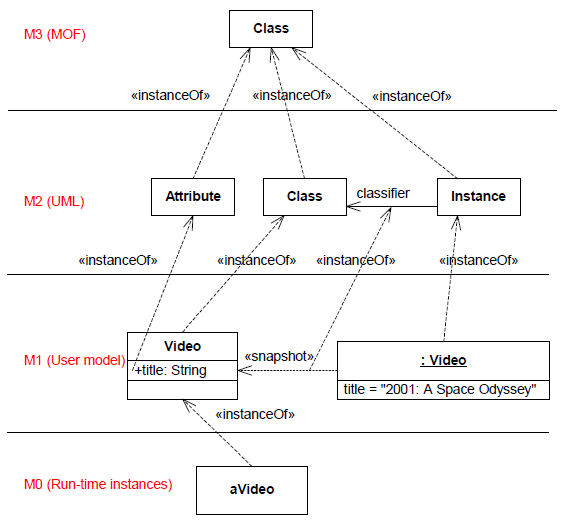
\includegraphics[width=\textwidth]{part2/umlMetalevels.png}
		\caption{Иерархия метаописаний UML, из \cite{omg2011infrastructure}.}
		\label{umlMetalevels}
	\end{center}
\end{figure}

Интересно то, что некоторые сущности языка UML существуют одновременно на нескольких 
уровнях метаописаний, например, классификаторы (абстракция способа классификации экземпляров) 
являются, с одной стороны, базой для определения понятия "`класс"' диаграммы классов 
(на уровне метамодели UML), с другой стороны, они же служат базой для определения 
классов и отношений в самом метаязыке (в пакете Core::Constructs). Кроме того, в стандарте 
UML определена только та часть метаязыка MOF, которая нужна для описания метамодели UML, 
сам MOF определяется отдельным стандартом, так что формально неверно то, что UML определён 
с помощью MOF. Всё это делает метамодель UML весьма запутанной, сложной для изучения 
и для переиспользования при создании предметно-ориентированных языков. 

Поэтому язык UML включает в свой стандарт механизм легковесного расширения, называемый 
профилями. Профили позволяют расширить существующие метаклассы из метамодели UML, 
чтобы адаптировать язык под нужды конкретной предметной области. Достигается это путём 
определения стереотипов --- "`ограниченных"' метаклассов, которые могут быть применены 
к уже существующим метаклассам для того, чтобы дополнить их новыми свойствами или 
поменять их изображение. Например, метакласс "`класс"' может быть расширен стереотипом 
"`часы"', имеющим свойства "`количество кнопок"', "`тип операционной системы"' и специальную 
иконку для отображения. Генераторы, умеющие работать с определённым профилем, могут, 
во-первых, различать метаклассы с разными стереотипами, во-вторых, использовать их 
дополнительные атрибуты. Благодаря этому можно довольно простым и стандартным образом 
описывать предметно-ориентированные языки на базе UML. Однако же, профили позволяют 
только расширить язык UML, и сложность языка при использовании профилей всё равно 
сохранится. Вместе с тем, профили не позволяют определять новые сущности в метамодели. 
Профили, тем не менее, активно используются для генерации полного исходного кода, 
в том числе, в рамках подхода MDA~\cite{swithinbank2005patterns}.

В работе Аткинсона и Кюне \cite{atkinson2003model} приводится критика подхода, применённого в разработке UML, 
основанная на том, что четырёхуровневая архитектура метауровней не делает разницы между отношениями 
"`является лингвистическим экземпляром"' и "`является онтологическим экземпляром"'. 
Например, объект является экземпляром класса онтологически (то есть по смыслу), но 
формально диаграммы объектов и диаграммы классов не связаны. UML использует одно и 
то же отношение instanceOf как для обозначения того, что некоторая модель является 
экземпляром метамодели (лингвистическая связь), так и сугубо на уровне модели, для 
обозначения того, что объект является экземпляром класса. Автор предлагает явно разделить 
эти два варианта отношения instanceOf, и ввести кроме лингвистической понятие онтологической 
метамодели. Таким образом, фактически, получится обобщение механизма профилей, позволяющее
более адекватно выражать отношения предметной области. В качестве примера автор приводит 
зоологическую классификацию животного мира: класс "`Колли"' является наследником класса 
"`Собака"', при этом онтологическим экземпляром класса "`Порода"'. Класс "`Собака"' 
является онтологическим экземпляром класса "`Вид"'. И "`Порода"', и "`Вид"' --- онтологические 
экземпляры класса "`Биологический ранг"'.

Идеи Кюне и Аткинсона были реализованы в системе MetaDepth~\cite{de2010deep, de2012domain}. Платформа позволяет описывать
только текстовые предметно-ориентированные языки, что не позволяет нам рассматривать её в обзоре вместе с другими DSM-платформами,
но упоминания здесь она всё же заслуживает. Система позиционируется как платформа для "`глубокого метамоделирования"'
и предназначена прежде всего для создания метамоделей предметно-ориентированных языков с использованием как лингвистического,
так и онтологического инстанциирования. Описываемый язык может иметь произвольное количество метауровней 
(не просто "`метаязык-метамодель-модель"', как в UML, а серия моделей, каждая из которых может быть
моделью, описанной на языке более высокого метауровня, и одновременно метамоделью для более низкого метауровня). Такой
подход позволяет естественно выражать отношения "`тип-экземпляр"', возникающие, например, между диаграммами 
классов и диаграммами объектов в UML. Метамодель задаётся в текстовой форме, имеются средства для описания
конкретного синтаксиса языков, ограничений и трансформаций моделей, все они учитывают то, что иерархия метамоделей "`глубокая"'. 
Авторы приводят примеры нескольких предметно-ориентированных языков, построенных по такому принципу, имеется 
работающий прототип системы в свободном доступе.

\section{Создание визуальных языков в существующих DSM-платформах}
\subsection{Платформа MetaEdit+}
Наиболее зрелой и известной на данный момент DSM-платформой является среда MetaEdit+, 
разрабатываемая финской компанией MetaCase, на базе научного проекта University of Jyvaskyla. 
Среда MetaEdit, из которой развилась среда MetaEdit+, создавалась с 1988 года, впоследствии 
была существенно переработана, и сейчас она (точнее, MetaEdit+) --- успешный коммерческий проект, 
имеющий десятки внедрений и активно публикующийся по своим результатам (\cite{kelly2008domain, luoma2004defining, tolvanen2007advanced, tolvanen2009metaedit}). 
Впрочем, исходный код системы закрыт, а лицензия довольно дорогая, что делает затруднительным 
переиспользование результатов проекта для дальнейших исследований другими научными группами.

Система состоит из двух компонент: MetaEdit+ Workbench и MetaEdit+ Modeler. Первая 
предназначена для создания предметно-ориентированных визуальных языков, вторая --- для 
их использования. В качестве метаязыка система использует собственный язык GOPPRR. 
Его название образовано первыми буквами основных понятий, в нём используемых: граф (graph), 
объект (object), свойство (property), порт (port), отношение (relation), роль (role). 
Граф служит для представления модели (или диаграммы), в графе могут содержаться объекты, 
отношения и роли. Объект --- это сущность предметной области (вершина графа), отношение 
связывает два или несколько объектов, при этом отношения соединяются с объектами с помощью ролей. 
Например, отношение наследования может иметь роли "`предок"' и "`потомок"', роль "`предок"' 
рисуется в виде линии с треугольником на конце, роль "`потомок"' в виде простой линии, 
а само отношение (это может показаться неинтуитивным) не визуализируется. Роли могут 
соединяться с самими объектами, а могут соединяться с портами --- специальными областями 
внутри объектов, которые различаются генераторами и нужны, если одна и та же роль может 
иметь разные значения в зависимости от того, к какой части объекта подключена. Так, 
например, удобно моделировать различные приборы: объект "`Усилитель"' может иметь аналоговый 
вход, цифровой вход и аналоговый выход. Свойства --- это некоторые характеристики 
(вида "`имя"'-"'значение"'), которыми могут обладать все остальные понятия. Кроме 
этого, в метаязыке присутствуют понятия Binding (связывает отношения, роли и объекты),
Object set (множество объектов, играющее одну роль, например, в Binding-е), Inheritance 
(отношение наследования между метатипами), Decomposition (возможность задать раскрытие 
какого-либо объекта в подграф, например, класс, раскрывающийся в диаграмму автоматов) и 
Explosion (возможность связывать объекты, отношения или роли с другими графами).

Предлагаемая этой DSM-платформой методика создания языка такова: сначала определяются 
основные концепции языка (сущности и связи), затем задаются ограничения, определяются 
графические символы для концепций, затем определяются правила генерации. Процесс итеративен, 
все изменения, вносимые в метамодель, тут же применяются к модели. Если вносимое в метамодель 
изменение конфликтует с существующими моделями, выдаётся предупреждение. Существует визуальный 
язык для задания метамодели, но его использование не обязательно, причём в документации и 
обучающих материалах визуальный язык, как правило, не используется --- метамодель редактируется 
с помощью диалоговых окон. Метамодель можно до определённой степени менять прямо из редактора 
модели: задавать сущностям новые свойства, менять существующие, редактировать их внешний 
вид. Однако добавить новую сущность в язык или удалить существующую можно только через 
редактор метамодели. Поскольку изменения в метамодели тут же отражаются в редакторе модели, 
это позволяет организовать работу над языком короткими итерациями с непосредственным 
участием эксперта, как в случае с AgentSheets, но пользовательский интерфейс MetaEdit+ 
довольно сложен, что требует наличия подготовленного специалиста по созданию языков. 
Инструмент непосредственно поддерживает только создание и изменение языка, в работах авторов 
имеются методологические рекомендации по действиям в других фазах жизненного цикла, но 
непосредственно в инструментарии они не поддержаны.

\subsection{Eclipse Modeling Project}
Ещё одна DSM-платформа, ставшая стандартом де-факто для исследований в области предметно-ориентированного визуального моделирования --- 
%TODO: ссылка!
Eclipse Modeling Project (EMP). Фактически, это объединение большого количества различных библиотек и инструментов, часть которых развивается 
независимо и предназначается не только для визуального моделирования. Проект строится на базе платформы 
%TODO: ссылка
Eclipse, имеет открытый исходный код и большое сообщество разработчиков. На базе этого 
проекта существует несколько коммерческих инструментов, например, DSM-платформа Borland Together
\footnote{Сайт Borland, Домашняя страница Borland Together, URL: http://www.borland.com/products/together/ (дата обращения 02.06.2013)}
, CASE-система Rational Software Architect
\footnote{Сайт IBM, Информация о продукте Rational Software Architect, 
URL: http://www-03.ibm.com/software/products/us/en/ratisoftarch (дата обращения 02.06.2013)}
, DSM-платформа Obeo Designer
\footnote{Сайт Obeo Designer, URL: http://www.obeodesigner.com/ (дата обращения 14.06.2014)}
, а также несколько исследовательских проектов в области предметно-ориентированного моделирования, например, MOFLON
%TODO: Ссылка 
. При этом проект активно развивается, появляются новые библиотеки и средства создания предметно-ориентированных 
языков (например, библиотека для создания графических редакторов Graphiti 
\footnote{Домашняя страница проекта Graphiti на сайте Eclipse, URL: http://www.eclipse.org/graphiti/ (дата обращения 02.06.2013)}
и генератор редакторов по текстовому описанию Spray
\footnote{Домашняя страница проекта Spray на Google Code, URL: https://code.google.com/a/eclipselabs.org/p/spray/ (дата обращения 02.06.2013)}
, построенный поверх этой библиотеки). Это создаёт большие сложности в использовании и изучении этого проекта, поскольку имеющаяся документация 
фрагментарна и сильно отстаёт от ведущейся разработки, публикации, как правило, посвящены 
отдельным подпроектам, и имеется лишь немного материала, посвящённого проекту в целом 
(например, \cite{gronback2009eclipse}, и статья на русском языке \cite{sorokin2010obzor}).

В качестве метаязыка в EMP используется язык Ecore, который представляет собой близкую 
к стандарту реализацию MOF (точнее, его варианта EMOF), метаязыка UML. Элемент создаваемого 
языка представляется в метамодели объектом метакласса EClass, у него могут быть атрибуты, 
задаваемые объектами метакласса EAttribute, операции, задаваемые объектами EOperation, и 
ассоциации, задаваемые объектами EReference. Атрибуты имеют тип, моделируемый с помощью 
метакласса EDataType. Кроме того, имеется возможность добавлять аннотации элементам 
(которые могут быть использованы при генерации), с помощью метакласса EAnnotation.

Процесс разработки предметно-ориентированного языка, предполагаемый при использовании GMP, 
следующий: сначала создаётся проект плагина в Eclipse, затем в этом проекте определяется 
модель абстрактного синтаксиса (метамодель), модель конкретного синтаксиса, преобразования 
моделей в модели и моделей в текст (если требуется), текстовый конкретный синтаксис 
(если требуется), по результатам генерируются редакторы, генераторы и прочие инструменты, 
тестируются, процесс повторяется итеративно. По окончании разработки плагин-редактор 
дополняется различными мастерами, графикой и т.д., формируется инсталляционный пакет.

Абстрактный синтаксис языка может быть задан с помощью графической метамодели, либо 
импортирован из XSD-схемы, диаграммы классов UML, или даже исходного кода на Java. 
Это оказывается довольно удобным, поскольку позволяет переиспользовать существующие 
наработки: например, для языков, базирующихся на XML, XSD-схемы часто доступны как 
часть стандарта. Однако по метамодели средствами EMF могут быть сгенерированы только 
заглушки для классов предметной области, механизм оповещений об изменениях в модели, 
и простой редактор, представляющий модель в виде дерева. Конкретный синтаксис задаётся
с помощью библиотеки GMF, которая сама создавалась как отдельная DSM-платформа, и использует 
предметно-ориентированный подход к разработке. Для задания формы фигур надо создать 
модель определения графики (Graphical definition model). Для описания палитры элементов 
и панелей инструментов, используемых в создаваемом визуальном редакторе, необходимо 
создать модель инструментов (Tooling model). После этого надо связать эти две модели 
с моделью абстрактного синтаксиса, созданной с помощью EMF, с помощью модели соответствия 
(Mapping model), и определить модель генерации (Generator model), где определить все 
оставшиеся необходимые для генерации редактора свойства. Редактирование всех моделей 
производится с помощью специально предназначенных для этого мастеров.

Определение текстового синтаксиса для создаваемых языков возможно с помощью компонент 
Xtext и TCS, первая из которых позволяет задавать синтаксис, используя EBNF
%TODO: ссылка
, вторая --- путём связывания элементов конкретного синтаксиса с элементами метамодели. Определение 
правил преобразования модели в модель или модели в текст возможно с помощью языков 
QVTи ATL. Такие преобразования могут использоваться для определения рефакторингов 
над моделями, миграции моделей (то есть для преобразования моделей, созданных в соответствии 
со старой версией метамодели, в модели, соответствующие новой метамодели), объединения 
двух или нескольких моделей в одну модель, или генерации кода на текстовых языках. 
Все преобразования описываются на текстовых языках. Есть и специальные средства для задания правил генерации (компоненты Xpand/Xtend
\footnote{Страница Xpand на Eclipse Wiki, URL: http://wiki.eclipse.org/Xpand (дата обращения 12.06.2013)}
), которые также в текстовом виде позволяют описывать правила генерации, в виде шаблонов кода на целевом языке, дополненных 
императивным языком, задающим правила обхода модели и генерации параметризуемых из модели 
фрагментов. Общая схема создания предметно-ориентированного решения в Eclipse Modeling 
Project представлена на рисунке~\ref{empProcess}.

\begin{figure} [ht]
	\begin{center}
		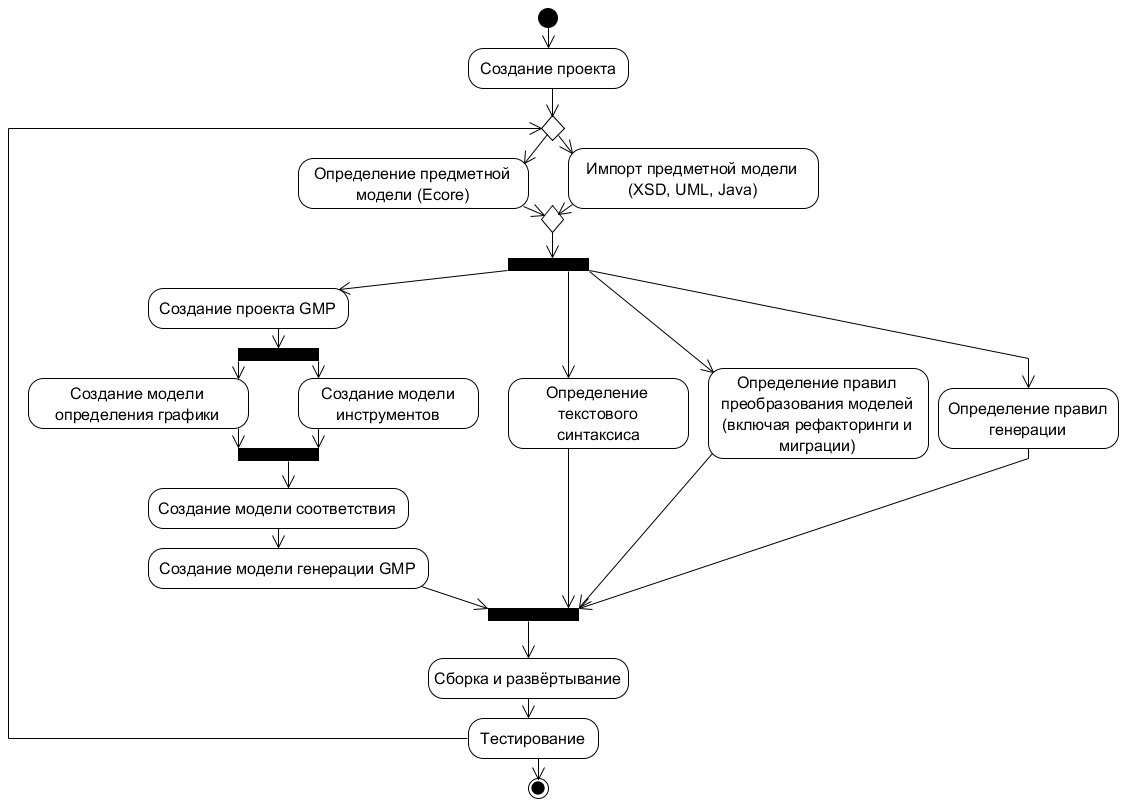
\includegraphics[width=0.9\textwidth]{part2/empProcess.png}
		\caption{Процесс создания DSM-решения на EMP.}
		\label{empProcess}
	\end{center}
\end{figure}

Как видно, процесс создания DSM-решений на EMP сложен сам по себе, и дополнительно 
усложняется слабой связностью наличествующих компонентов. Существует даже отдельный 
проект по объединению всего существующего в единую технологию (Modeling Amalgamation Project
\footnote{Домашняя страница Modeling Amalgamation Project на сайте Eclipse, URL:  http://www.eclipse.org/modeling/amalgam/ (дата обращения 12.06.2013)}
), однако новые компоненты продолжают появляться, технология активно развивается, и использование 
её всё ещё требует больших усилий на исследование и выбор доступных средств (далеко 
не все существующие в рамках EMP проекты достаточно зрелые для реального использования). 
Кроме того, наличествующие средства, помимо усилий на создание большого количества 
разных моделей и текстовых спецификаций, по которым будет сгенерировано DSM-решение, 
зачастую требуют и ручного кодирования на языке Java. Таким образом, EMP используется 
в основном как база для разработки более доступных для конечного пользователя инструментов.

\subsection{Платформа Generic Modeling Environment}
Платформа Generic Modeling Environment (GME)
\footnote{Домашняя страница GME, URL: http://www.isis.vanderbilt.edu/Projects/gme/ (дата обращения 12.06.2013)}
\cite{ledeczi2001generic} является одной из самых известных академических разработок в области создания DSM-решений. 
Эта платформа имеет расширяемую модульную архитектуру, благодаря чему на её основе было создано 
несколько исследовательских и промышленных инструментов (например, средство симуляции встроенных систем MILAN
\footnote{Домашняя страница MILAN, URL: http://w3.isis.vanderbilt.edu/projects/milan/ (дата обращения 12.06.2013)}
, средство для аспектно-ориентированного задания ограничений на модели C-SAW
\footnote{Домашняя страница C-SAW, URL: http://www.gray-area.org/Research/C-SAW/ (дата обращения: 12.06.2013)}
). Проект имеет открытый исходный код, разрабатывается в основном на языке C++, до сих пор развивается.

Визуальные языки в GME задаются с помощью визуальных метамоделей (авторы GME рассматривают 
задачу разработки визуального языка как просто ещё одну задачу, к которой может быть 
применён предметно-ориентированный подход). Метаязык ориентирован на иерархическую 
декомпозицию моделей: любой составной элемент языка является моделью сам по себе, и 
задаётся метаклассом Model. Элементы, которые не могут иметь составных частей, называются 
атомами (метакласс Atom). Модель может состоять из подмоделей и атомов, при этом каждый 
атом внутри модели имеет роль (метакласс Role): роли задают "`гнёзда"' внутри модели, 
куда пользователь может вставлять различные подмодели и атомы. Управление отображением 
частей модели осуществляется с помощью метакласса Aspect --- каждая модель имеет предопределённый 
набор аспектов, каждая часть может быть видима или скрыта в каком-либо аспекте. Каждая 
сущность языка имеет набор "`основных"' аспектов, в которых она может быть создана 
или удалена. Связи между объектами задаются с помощью метакласса Connection. Связываемые 
элементы модели должны иметь одного родителя в иерархии вложенности и быть одновременно 
видимыми в одном аспекте. Если требуется связать элементы, относящиеся к разным моделям, 
используются невизуальные ссылки, описываемые в метамодели метаклассом Reference. Ссылка 
выглядит как обычный объект, и может использоваться в какой-либо роли в модели, но на 
самом деле она представляет объект, находящийся где-то ещё, по аналогии со ссылками 
или указателями в текстовых языках программирования. Возможно также определение N-арных 
отношений, задаваемых в метамодели метаклассом Set. Отношения, атомы, ссылки, связи, 
модели могут иметь атрибуты, задаваемые метаклассом Attribute, и ограничения, задаваемые 
метаклассом Constraint. Ограничения задаются на стандартном языке OCL. Модели могут 
быть организованы в папки (описываемые на уровне метамодели метаклассом Folder), папки 
могут содержаться в проекте (метакласс Project).

Возможно переиспользовать существующие метамодели при разработке новых, для этого 
используются ссылки и операторы, определённые в метаязыке: эквивалентность, наследование 
реализации и наследование интерфейса. Оператор эквивалентности связывает два класса 
и делает их одним, объединяя все атрибуты, операции и связи двух классов. С помощью 
оператора эквивалентности можно создавать “точки склейки” между разными метамоделями. 
Различные операторы наследования введены для более точного управления наследованием 
отношений, в которых участвует наследуемый класс: в случае наследования реализации 
наследуются все атрибуты класса и те отношения вложенности, в которых наследуемый 
класс участвует как контейнер; в случае наследования интерфейса, наоборот, атрибуты 
не наследуются, но наследуются все отношения, в которых участвует класс, кроме отношений 
вложенности, в которых наследуемый класс участвует как контейнер.

По созданной метамодели может быть автоматически сгенерирован предметно-ориентированный 
визуальный редактор, после чего его тут же можно начать использовать в среде. В качестве 
конкретного синтаксиса используется синтаксис диаграммы классов UML, который может 
быть расширен иконками и цветом. Специальных средств для задания правил генерации 
или преобразования моделей в среде нет, имеется развитый программный интерфейс, с 
помощью которого авторы DSM-решений могут реализовать свои инструменты. Именно так 
реализован генератор редакторов самого GME --- отдельный плагин, который работает с 
метамоделью через API, и генерирует файл с описанием парадигмы (собственно, предметно-ориентированного 
редактора), который потом может быть загружен в среду. Такой подход, хоть и позволяет 
обеспечить достаточно быстрое прототипирование визуального языка, требует знания API GME 
и существенных усилий в "`ручном"' программировании, чтобы создать полноценное решение. 
Автоматическая миграция моделей при изменении метамоделей также не поддерживается, 
таким образом, эволюцию предметно-ориентированного решения приходится организовывать также вручную. Существует отдельный проект GReAT
\footnote{Домашняя страница GReAT, URL: http://www.isis.vanderbilt.edu/tools/GReAT (дата обращения 12.06.2013)}
, предоставляющий возможности для описания преобразования моделей в GME.

\subsection{Платформа AToM3}
Платформа AToM\textsuperscript{3}
\footnote{Домашняя страница AToM\textsuperscript{3}, URL: http://atom3.cs.mcgill.ca/ (дата обращения 12.06.2013)}
--- это ещё один пример академической разработки, предназначенный прежде всего для изучения преобразования моделей. Проект имеет открытые 
исходные коды, реализован на языке Python, отличается нестабильностью и неудобностью пользовательского интерфейса
%TODO: субъективно
, тем не менее, широко известен в научном сообществе, имеется большое количество публикаций (например, \cite{vangheluwe2004domain}).
%TODO: ещё ссылки на публикации
Ныне не развивается, авторы использовали полученный опыт при разработке системы MetaDepth, описанной выше.

В качестве метаязыка в AToM\textsuperscript{3} используется язык "`сущность-связь"', позволяющий в виде 
сущностей с атрибутами задавать сущности предметной области, и в виде связей описывать 
взаимосвязи между ними. Имеется также несложный векторный редактор, позволяющий описывать 
конкретный синтаксис элементов. По описанию метамодели генерируется код редактора 
на языке Python, после чего редактор может быть загружен в среду. 

Каждая метамодель может быть снабжена набором трансформаций, описываемых с помощью 
графовых грамматик. Грамматика состоит из продукций, каждая из которых имеет левую 
часть (шаблон, который ищется в исходном графе), правую часть (то, на что надо заменить 
найденный шаблон), условие применения (логическое выражение на языке Python, продукция 
применяется только если оно истинно) и действие, выполняемое после применения продукции 
(тоже код на языке Python). В продукции можно указать соответствие между элементами 
левой и правой части, что позволяет копировать или модифицировать свойства, кроме 
того можно создавать или удалять узлы. С помощью таких преобразований можно определять 
операционную семантику языка, либо давать возможность преобразовать модель в модель 
на другом языке. Таким же образом реализуется и кодогенерация: графовая грамматика 
задаёт продукции, не совершающие содержательных преобразований, а код на текстовом 
языке генерируется как побочные эффекты выполнения правил.

Таким образом, цикл разработки DSM-решения на AToM\textsuperscript{3} состоит из определения метамодели 
языка, определения конкретного синтаксиса, определения правил преобразования моделей, 
генерации редактора и тестирования. Однако, среда недостаточно зрела для промышленного 
использования и подходит только для разработки прототипов.

\subsection{Платформа Microsoft Modeling SDK}
Технология Microsoft Modeling SDK~\cite{cook2007domain} более известна в научном сообществе как Microsoft DSL Tools,
и с начала своего существования (2003 г.) успела несколько раз сменить название. Технология является
подключаемым модулем к среде разработки Microsoft Visual Studio\footnote
{Домашняя страница Microsoft Visual Studio, URL: http://www.visualstudio.com/ (дата обращения: 11.08.2014)}
и доступна для бесплатного скачивания с сайта Microsoft. Среда позволяет прямо в Visual Studio
в графическом виде задать метамодель создаваемого языка, описать внешний вид элементов, 
задать в текстовом виде правила генерации и ограничения и сгенерировать подключаемый модуль с
редактором языка и генератором, который можно запустить в Visual Studio. Технология требует установленной 
Visual Studio и для создания, и для использования предметно-ориентированных решений.
Тем не менее, зрелость технологии и хорошая интеграция её в Visual Studio делают её
весьма привлекательной для промышленных разработчиков.

Метамодель задаётся на метаязыке, напоминающем диаграммы классов UML --- поддерживаются
отношения между сущностями, свойства сущностей, наследование как сущностей, так и связей.
Интересной особенностью метаязыка является то, что метамодель рисуется всегда в виде дерева,
упорядоченного по связям между сущностями (вложенность или наличие связи), и если граф метамодели
не допускает представление в виде дерева (как, например, при наличии циклических отношений),
одну сущность нужно разместить на диаграмме метамодели несколько раз. Конкретный синтаксис
задаётся для каждой сущности посредством выбора из доступных в визуальном редакторе Visual Studio
примитивов, и описывается на той же диаграмме, что и абстрактный синтаксис --- диаграмма
разделена на две части, и сущности в абстрактной метамодели соединены линиями с описаниями их конкретного синтаксиса.
При желании форму фигур можно сделать произвольной, но это требует ручного кодирования на языке C\#.

Правила генерации кода на текстовом языке задаются с помощью шаблонов на языке Т4, которые
представляют собой текст на целевом языке со вставками конструкций, управляющих процессом 
генерации, на языке C\# (похожий подход применяется в технологии Microsoft ASP.NET\footnote
{Домашняя страница ASP.NET, URL: http://www.asp.net/ (дата обращения 11.08.2014)}
для генерации HTML-страниц). В управляющих конструкциях есть доступ к элементам модели, кроме того,
есть возможность описывать произвольный код генератора внутри шаблона. Ограничения на модели
описываются целиком на языке C\# с использованием довольно развитой инфраструктуры для
проверки ограничений, они могут проверяться как непосредственно при рисовании диаграммы
на предметно-ориентированном языке, так и при сохранении диаграммы (если диаграмма 
неконсистентна, будет выдано предупреждение, и генератор не запустится). С помощью этого
же механизма могут быть реализованы дополнительные инструменты работы с моделями, например,
поддержка рефакторингов.

В книге~\cite{cook2007domain} приводится ряд рекомендаций по процессу создания языка.
Первое, что надо сделать по мнению авторов --- выявить изменяемые части предметной области,
которые и будут задаваться визуальным языком. Для этого авторы предлагают использовать
деревья функциональности (feature trees\footnote{см. K. Czarnecki, S. Helsen, U. Eisenecker, `"Staged Configuration
Using Feature Models'" Software Product Lines: Third International Conference, Boston, MA, 2004}),
метод, очень похожий на метод FODA, один из формальных методов, упоминавшихся в~\ref{lifecycleModels}.
Для разработки метамодели авторы предлагают использовать наброски диаграмм на создаваемом языке
для рассмотрения конкретных сценариев его применения и выделения наиболее изменчивых частей.
Данные методы предлагается использовать неформально, инструментальной поддержки для них не предусмотрено.
Для определения правил генерации предлагается инкрементальный подход --- сначала код модельного
приложения копируется в шаблон без изменений, потом некоторые его части замещаются правилами генерации
по модели, на каждом этапе генерируется предметно-ориентированное решение и проверяется
его работоспособность.

В целом, технология производит впечатление достаточно зрелой, но требующей большого
объёма ручного кодирования и знания составляющих её библиотек. 

\subsection{Платформа Pounamu}
Платформа Pounamu~\cite{zhu2007pounamu} создавалась как DSM-платформа для разработки 
многопользовательских визуальных сред разработки, способных использовать одновременно 
несколько нотаций для одного языка. В основу архитектуры системы были заложены принципы 
простоты использования (то есть простоты задания визуального языка и определения инструментальной 
поддержки для него) и простоты расширения и модификации. Платформа имеет довольно 
гибкую архитектуру, включающую в себя API в виде веб-сервисов и сериализацию создаваемых 
моделей в виде XML-файла, что позволяет удобно создавать инструменты, расширяющие её 
функциональность. В частности, благодаря этому была реализована функциональность просмотрщиков 
моделей в браузере и на мобильном телефоне.

Pounamu обладает довольно развитыми метасредствами, включающими в себя визуальный 
метаредактор, визуальный редактор формы фигур, визуальный редактор обработчиков событий. 
В качестве метаязыка используется язык "`сущность-связь"', с интересной особенностью: 
ассоциации в метамодели соединяют элементы, экземпляры которых будут соединять в модели 
экземпляры этих ассоциаций, например, отношение “реализует” между классом и объектом 
является отношением между метаклассами "`класс"' и "`объект"' в метамодели. Авторы 
намеренно сделали метаязык очень простым, чтобы он был доступен возможно более широкому 
кругу пользователей. На метаязыке описывается только абстрактный синтаксис языка, для 
задания конкретного синтаксиса существует редактор формы фигур, при этом связь между 
формами, созданными с помощью этого редактора, и элементами метамодели осуществляется 
с помощью модели соответствия, которая позволяет задавать несколько форм для одного 
элемента, указывать, как поля на форме соответствуют свойствам элемента в метамодели 
и т.д. Для того, чтобы задать, какую из форм элемента использовать в конкретном контексте, 
используется понятие "`вид"' (близкое к понятию "`диаграмма"' языка UML), с помощью 
диалогового редактора можно указать, какие формы элементов используются в каком виде.

Заслуживает особого внимания способ реализации сложной логики средств инструментальной 
поддержки (например, проверки ограничений, генерации, задания сложных правил отображения 
между элементами метамодели и формами элементов, автоматического размещения элементов 
на диаграммах). Для этого используется визуальный язык задания правил обработки событий, 
напоминающий язык SDL или блок-схемы. В DSM-решении могут происходить различные события 
(например, создание или перемещение элемента, нажатие кнопки на панели инструментов), 
обработчик может подписываться на событие и выполнять некоторые действия, состоящие из 
довольно высокоуровневых команд системы. Имеется визуальный отладчик обработчиков. 
Имеется возможность определять свои блоки для диаграмм обработчика программированием 
на языке Java. При этом DSM-платформа обеспечивает динамическую компиляцию и загрузку 
написанного кода прямо в процессе работы.

Предлагаемая авторами методология разработки предполагает быстрое итеративное создание 
языка, с немедленным тестированием вносимых изменений, без длительной перекомпиляции 
и перезапуска платформы. Сначала описывается конкретный и абстрактный синтаксисы, 
модель соответствия, затем определяется логика инструментальных средств с помощью 
редактора обработчиков событий. При необходимости код на Java дописывается вручную. 
Возможно дальнейшее расширение инструментальной поддержки ручным кодированием с использованием 
API веб-сервисов или разбором XML-файлов с сохранёнными моделями. Таким образом, методология 
предполагает ручное программирование на поздних этапах разработки. Кроме того, даже 
ограничения или рефакторинги в Pounamu задаются с помощью языка обработки событий 
(по сути, низкоуровневого языка общего назначения).

\subsection{Платформа DOME}
Платформа DOME~\cite{engstrom2000building, guide1999honeywell} (DOmain Modeling Environment) создавалась с целью упростить
прототипирование и создание графических модельно-ориентированных сред разработки. Это одна из первых
DSM-платформ с поддержкой графического описания метамодели визуального языка, разрабатываемая 
компанией Honeywell с 1992 года. Платформа имеет возможность как генерировать по метамодели редактор
визуального языка на языке Smalltalk, так и интерпретировать метамодель напрямую. Для
задания ограничений, правил генерации, трансформации моделей и настройки поведения элементов 
используется специальный текстовый язык Alter (диалект Scheme
\footnote{Стандарт Scheme R6RS, URL:http://www.r6rs.org/ (дата обращения 14.06.2014)}
), либо визуальный язык Projector. Есть и упрощённый генератор документации, позволяющий задавать шаблон документации в виде
.doc-файла, где размечены места, заполняемые генератором по модели.

Метаязык, используемый в DOME, называется DTSL (DOME Tool Specification Language) и реализован в 
метаредакторе в самой системе, называемом ProtoDome. Язык представляет собой вариант диаграмм "`сущность-связь"', позволяет задавать узлы языка,
связи между ними, ограничения на связи, правила структурной декомпозиции диаграмм
(какой узел может содержать какую диаграмму в качестве подэлемента). Большое внимание
в метаязыке уделяется графической нотации создаваемого языка --- большая часть редактируемых свойств
относится именно к конкретному синтаксису. Связано это с тем, что DOME не имеет встроенного
редактора конкретного синтаксиса, поэтому настройка внешнего вида элементов выполняется через
свойства элементов в метаязыке, либо ручным кодированием на Alter. Такой подход, тем не менее,
достаточно удобен, поскольку DOME предоставляет много возможностей по настройке внешнего вида элементов,
а наличие прямо в метаязыке таких сущностей, как, например, "`Палитра"' или "`Список свойств"' позволяет быстро
и эффективно создавать редакторы, не прибегая к ручному кодированию или использованию вспомогательных
инструментов. Визуальный метаязык хорошо интегрирован с текстовым языком Alter, каждый
элемент метаязыка имеет набор свойств --- программ на Alter, которые вызываются средой при 
наступлении события, соответствующего свойству.

Предлагаемый подход к разработке языка состоит в описании метамодели языка в DOME и последующей
её интерпретации, создании модели с её помощью и внесении изменений в метамодель "`на лету"',
при этом среда автоматически обновляет все имеющиеся в репозитории модели и открытые редакторы.
Сами авторы отмечают в \cite{guide1999honeywell}, что такие действия могут приводить к 
неконсистентности моделей, например, при изменении типа свойства, причём это не отслеживается средой.
Кроме того, среда не сохраняет в модели значения свойств по умолчанию, так что изменение их в
метамодели может привести к неожиданным для пользователей изменениям в модели. При
этом для изменения метамодели требуется наличие метаредактора. После того, как метамодель
будет завершена, к ней возможно написать генератор, либо на Alter или Projector, либо используя
упрощённый генератор MetaScribe. Также есть возможность задать трансформации моделей, 
дополнительные ограничения, определить свои инструменты, которые будут добавлены на палитру,
всё это делается на Alter или Projector, то есть языках общего назначения.

\section{Выводы}
Выполненный обзор научных публикаций по методологиям и технологиям создания предметно-ориентированных 
языков выявил недостаток внимания со стороны исследователей к технологиям, связанным 
с визуальными языками. Существующие работы либо подробно описывают методологию создания 
предметно-ориентированных языков, но ориентированы только на текстовые языки, либо 
описывают инструменты для создания предметно-ориентированных визуальных языков, но 
практически без методологической поддержки, причём очень часто внимание уделяется 
только самой реализации визуального языка. Таким образом, если автор DSM-решения уже 
"`знает, что писать"' (то есть имеет в голове ясное представление о предметной области 
и даже метамодель создаваемого языка), то к его услугам множество существующих инструментов. 
Но если требуется вести разработку предметно-ориентированного решения "`с нуля"' (начиная 
с оценки осуществимости и анализа предметной области), очень многое придётся делать 
без какой-либо инструментальной поддержки и, как правило, без руководства к действию. 
Поэтому сейчас создание DSM-решений требует немалой квалификации и опыта даже при 
использовании промышленных средств, таких как MetaEdit+.

Таким образом, явно имеется пробел в существующих исследованиях, который данное исследование
призвано помочь заполнить. Наиболее близкой по содержанию к данной диссертации является
рассмотренная в обзоре работа \cite{repenning1995agentsheets}, где предлагается методология
коллаборативной разработки визуального языка и технология её поддержки. Однако эта
методология применима лишь для довольно узкого класса языков и в относительно несложных
случаях. Другие существующие технологические средства сконцентрированы на решении
своих узких задач и не предназначены для поддержки полного цикла разработки языка.
Многие из них реализуют только одну конкретную составляющую предметно-ориентированного
решения, что, если вспомнить о практически полном отсутствии возможностей для интеграции
между инструментами различных производителей, делает возможным только прототипирование
DSM-решений.
